%! suppress = EscapeHashOutsideCommand
%! suppress = Quote
%! suppress = MissingImport
%! suppress = MissingLabel
%! suppress = LineBreak

% CLI args https://tex.stackexchange.com/a/1501
\newif\ifhandout
\input{flags}

%! suppress = MissingLabel
%! suppress = DocumentclassNotInRoot
%! suppress = DiscouragedUseOfDef

% * Make friends tikz & colors
%   https://en.wikibooks.org/wiki/LaTeX/Colors
% * To enable vertical top alignment globally
%   https://tex.stackexchange.com/questions/9889/positioning-content-at-the-top-of-a-beamer-slide-by-default
% * Set handout from CLI
%   https://tex.stackexchange.com/a/1501
\ifhandout
\documentclass[usenames, dvipsnames, handout]{beamer} % https://tex.stackexchange.com/questions/224091/beamer-how-to-disable-pause-temporarily
\else
\documentclass[usenames, dvipsnames]{beamer}
\fi
% ------------------------------------------------

% Graphics
\usepackage{color}
\usepackage{tabularx}
\usepackage{tikz}
% https://tikz.dev/tikz-graphs
\usetikzlibrary{positioning, shapes.geometric, arrows, automata, graphs}
\tikzset{
    expr/.style={ellipse, draw=gray!60, fill=gray!5, very thick, minimum size=7mm, yshift=0.7cm},
    hexpr/.style={ellipse, draw=gray!60, fill=blue!15, very thick, minimum size=7mm, yshift=0.7cm},
    stmt/.style={rectangle, draw=gray!60, fill=gray!5, very thick, minimum size=5mm, yshift=0.7cm},
    decl/.style={rectangle, draw=blue!60, fill=gray!5, very thick, minimum size=5mm, yshift=0.7cm},
    hdecl/.style={rectangle, draw=blue!60, fill=blue!15, very thick, minimum size=5mm, yshift=0.7cm},
    subtree/.style={shape border rotate=90, isosceles triangle, draw=gray!60, fill=gray!5, very thick, minimum size=5mm, yshift=0.0cm},
}
\usepackage{blkarray}
\usepackage{graphicx}
\usepackage{forest} % https://tex.stackexchange.com/questions/198405/how-to-change-the-color-of-subtrees-in-tikz-qtree
% ------------------------------------------------

% Math
\usepackage{amsmath, amsfonts}
\usepackage{amssymb}
\usepackage{proof}
\usepackage{mathrsfs}
% Crossed-out symbols
% https://tex.stackexchange.com/questions/75525/how-to-write-crossed-out-math-in-latex
\usepackage[makeroom]{cancel}
\usepackage{mathtools}
% ------------------------------------------------

% Additional font sizes
% https://www.overleaf.com/learn/latex/Questions/How_do_I_adjust_the_font_size%3F
\usepackage{moresize}
% Additional colors
% https://www.overleaf.com/learn/latex/Using_colours_in_LaTeX
\usepackage{xcolor}
% Textual math symbols
\usepackage{textcomp}
% ------------------------------------------------

% Language
\usepackage[utf8] {inputenc}
\usepackage[T2A] {fontenc}
\usepackage[english, russian] {babel}
\usepackage{indentfirst, verbatim}
\usetikzlibrary{cd, babel}
% ------------------------------------------------

% Fonts: https://sites.math.washington.edu/~reu/docs/latex_symbols.pdf
\usepackage{stmaryrd}
\usepackage{cmbright}
\usepackage{wasysym}
\usepackage[weather]{ifsym} % https://tex.stackexchange.com/questions/100424/how-to-use-the-ifsym-package
% https://tex.stackexchange.com/questions/615300/pdflatex-builtin-glyph-names-is-empty
\pdfmapline{=dictsym DictSym <dictsym.pfb}
\pdfmapline{=pigpen <pigpen.pfa}
\usepackage{dictsym}
% ------------------------------------------------

% Code
% * Needs -shell-escape build flag
%   https://tex.stackexchange.com/questions/99475/how-to-invoke-latex-with-the-shell-escape-flag-in-texstudio-former-texmakerx
% * Set build directory
%   https://tex.stackexchange.com/questions/339931/latex-minted-package-using-custom-output-directory-build
\usepackage{minted}
\setminted{xleftmargin=\parindent, autogobble, escapeinside=\#\#}
% ------------------------------------------------

% Template
\usetheme{CambridgeUS}
\usecolortheme{dolphin}
% https://tex.stackexchange.com/questions/231439/beamer-how-to-make-font-larger-for-page-numbers
\setbeamerfont{headline}{size=\scriptsize}
\setbeamerfont{footline}{size=\scriptsize}
% Remove heddline
% https://tex.stackexchange.com/questions/33146/how-could-i-remove-a-header-in-a-beamer-presentation
%\setbeamertemplate{headline}{}
% Slide sizes
% https://tex.stackexchange.com/questions/56768/how-to-set-a-small-default-font-size-with-beamer
%\geometry{paperwidth=140mm,paperheight=105mm} % 4:3
\geometry{paperwidth=168mm,paperheight=105mm} % 16:10
% Remove navigation bar
% https://stackoverflow.com/questions/3210205/how-to-get-rid-of-navigation-bars-in-beamer
\beamertemplatenavigationsymbolsempty
% ------------------------------------------------

% Bullets
% https://9to5science.com/change-bullet-style-formatting-in-beamer
% https://tex.stackexchange.com/questions/185742/i-need-to-change-color-of-beamer-itemize-and-subitem-separately
\setbeamertemplate{itemize item}{\scriptsize\raise1.25pt\hbox{\donotcoloroutermaths$\blacktriangleright$}}
\setbeamertemplate{itemize subitem}{\scriptsize\raise1.5pt\hbox{\donotcoloroutermaths$\blacktriangleright$}}
\setbeamertemplate{itemize subsubitem}{\tiny\raise1.5pt\hbox{\donotcoloroutermaths$\blacktriangleright$}}
\setbeamertemplate{enumerate item}{\insertenumlabel.}
\setbeamertemplate{enumerate subitem}{\insertenumlabel.\insertsubenumlabel}
\setbeamertemplate{enumerate subsubitem}{\insertenumlabel.\insertsubenumlabel.\insertsubsubenumlabel}
% ------------------------------------------------

% Table of contents format
% https://tex.stackexchange.com/questions/642927/format-table-of-contents-in-beamer
\setbeamertemplate{section in toc}{%
        {\color{blue}\inserttocsectionnumber.}
    \inserttocsection\par%
}
\setbeamertemplate{subsection in toc}{%
        {\color{blue}\hspace{1em}\scriptsize\raise1.25pt\hbox{\donotcoloroutermaths$\blacktriangleright$}}
    \inserttocsubsection\par%
}
\setbeamertemplate{subsubsection in toc}{%
        {\color{blue}\hspace{2em}\tiny\raise1.25pt\hbox{\donotcoloroutermaths$\blacktriangleright$}}
    \inserttocsubsubsection\par%
}
% ------------------------------------------------

% Misc
\usepackage{multicol}
\usepackage{hyperref}
\usepackage{soul} % https://tex.stackexchange.com/questions/23711/strikethrough-text
% ------------------------------------------------

% Fix \pause for amsmath package envs (black black magic)
% https://tex.stackexchange.com/questions/16186/equation-numbering-problems-in-amsmath-environments-with-pause/75550#75550
% https://tex.stackexchange.com/questions/6348/problem-with-beamers-pause-in-alignments
%! suppress = Makeatletter
\makeatletter
\let\save@measuring@true\measuring@true
\def\measuring@true{%
    \save@measuring@true
    \def\beamer@sortzero##1{\beamer@ifnextcharospec{\beamer@sortzeroread{##1}}{}}%
    \def\beamer@sortzeroread##1<##2>{}%
    \def\beamer@finalnospec{}%
}
%! suppress = Makeatletter
\makeatother
% ------------------------------------------------

% Sections
\newcommand{\sectionplan}[1]{\section{#1}%
    \begin{frame}[noframenumbering]{Содержание}
        \tableofcontents[currentsection]
    \end{frame}
}
\newcommand{\subsectionplan}[1]{\subsection{#1}%
    \begin{frame}[noframenumbering]{Содержание}
        \tableofcontents[currentsubsection]
    \end{frame}
}
% ------------------------------------------------

% Footnotes
\renewcommand{\thefootnote}{\arabic{footnote}}
\renewcommand{\thempfootnote}{\arabic{mpfootnote}}
% https://tex.stackexchange.com/questions/28465/multiple-footnotes-at-one-point
\usepackage{fnpct}
% ------------------------------------------------

% Links
% Colors also links on slide foot.
%\hypersetup{
%    colorlinks=true,
%    citecolor=blue,
%    linkcolor=blue,
%    urlcolor=blue
%}
% ------------------------------------------------

% Appendix
% Slide numbers
% https://tex.stackexchange.com/questions/70448/dont-count-backup-slides
\usepackage{appendixnumberbeamer}
\newcommand{\backupbegin}{
    \newcounter{framenumbervorappendix}
    \setcounter{framenumbervorappendix}{\value{framenumber}}
}
\newcommand{\backupend}{
    \addtocounter{framenumbervorappendix}{-\value{framenumber}}
    \addtocounter{framenumber}{\value{framenumbervorappendix}}
}
% ------------------------------------------------

% Custom commands
% * Decor
\newcommand{\newtopic}[0]{$+$} % item: new topic on "in previous series"
\newcommand{\then}{$\Rightarrow$} % item: consequences
\newcommand{\pop}[0]{\SunCloud} %item:  general eduation
\newcommand{\popslide}[0]{(\pop)}
\newcommand{\advanced}[0]{$\varhexstar$} % item: advanced science
\newcommand{\advancedslide}[0]{(\advanced)}
\newcommand{\practical}[0]{\dstechnical} % item: practical programming notions
\newcommand{\practicalslide}[0]{(\practical)}
\newcommand{\todo}[0]{todo} % item: question
\newcommand{\answer}[0]{\Lightning} % item: answer to the previous question
\newcommand{\eg}[0]{e.g.} % item: example
\newcommand{\defi}[0]{$\Delta$} % item: definition on smth
\newcommand{\textdefi}[1]{\textbf{#1}}
\newcommand{\positive}{$+$} % item: pros
\newcommand{\negative}{{\color{red} $-$}} % item: cons
\newcommand%! suppress = EscapeHashOutsideCommand
\NB[1][0.3]{N\kern-#1em{B}} % default kern amount: -0.3em
\renewcommand{\emph}[1]{{\color{blue} \textit{#1}}}
\newcommand{\vocab}[1]{\textbf{#1}} % item: important new word
% * Lambda calculi
\newcommand{\comb}[1]{\mathbf{#1}} % defined combinator
\newcommand{\term}[1]{\mathbf{#1}} % predefined lambda-term reference
\newcommand{\termdef}{\coloneqq} % lamda term binding
\newcommand{\step}{\rightsquigarrow} % reduction step
\newcommand{\sstep}{\twoheadrightarrow} % multiple steps reduction
\newcommand{\ap}{~} % lambda-term application
\newcommand{\subst}[3]{\left[#2 \mapsto #3 \right] #1} % substitution
\newcommand{\eqbeta}{=_\beta} % beta equality
\newcommand{\eqeta}{=_\eta} % eta-equality
\newcommand{\eqt}{=} % tree-equality of terms
\newcommand{\tlist}[1]{\term{[}#1\term{]}} % list-term
% * Legacy
%\newcommand{\err}[0]{\textcolor{red}{ошибка}} % compilation error

% ------------------------------------------------

% Speaker notes
% https://tex.stackexchange.com/questions/114219/add-notes-to-latex-beamer
% https://tex.stackexchange.com/questions/35444/split-beamer-notes-across-multiple-notes-pages/35496#35496
%\setbeameroption{show notes on second screen=right} % enable speaker notes
%--------------------------------------

\author[]{Андрей Стоян, Илья Колегов, Дмитрий Халанский}
\institute[MSE ITMO]{MSE ITMO}


\title[8. Аппликативные функторы]{Практика 8. Аппликативные функторы}
\date{осень 2024}

\begin{document}

    \setcounter{framenumber}{-1}
    \maketitle

    \begin{frame}[fragile]{В предыдущих сериях}
        \begin{itemize}
            \item Полиморфные типы данных в Haskell (\mintinline{haskell}|Maybe|, \mintinline{haskell}|[]|, \mintinline{haskell}|Either|, \mintinline{haskell}|(->)|, \ldots)
            \item Функторы
            \item[\newtopic] Аппликативные функторы
        \end{itemize}
        \begin{center}
            
\includegraphics[width=0.6\textwidth]{figs/previous}
        \end{center}
    \end{frame}

    \begin{frame}[noframenumbering]{Содержание}
        \tableofcontents
    \end{frame}

    \sectionplan{Понимание классов типов}

    \begin{frame}[fragile]{Disclaimer}
        Понимание вещи --- чувство, иллюзия, состоящая из привыкания к ней и уверенности в себе.
        \begin{block}{``Понимание'' любого класса типов}
            \begin{itemize}
                \item Знать сигнатуры основных его функций
                \item Уметь использовать его функции на практике для типов-представителей
                \item Уметь писать реализации этого класса, удовлетворяющие его законам
                \item Уметь видеть на практике паттерны, которые им можно было бы абстрагировать
            \end{itemize}
        \end{block}
        \begin{block}{Всё остальное не обязательно!}
            \begin{itemize}
                \item Знать глубокий теоретический фундамент этого класса типов (даже если он есть)
                \item Чувствовать огромный набор интуиций, которые за ним стоят
                \begin{itemize}
                    \item Один из инструментов ``понимания''
                \end{itemize}
            \end{itemize}
        \end{block}
    \end{frame}

    \begin{frame}[fragile]{Зоопарк классов типов\footnote{Шпаргалка по зоопарку: {\color{blue}\url{https://wiki.haskell.org/Typeclassopedia}}.}}
        \begin{center}
            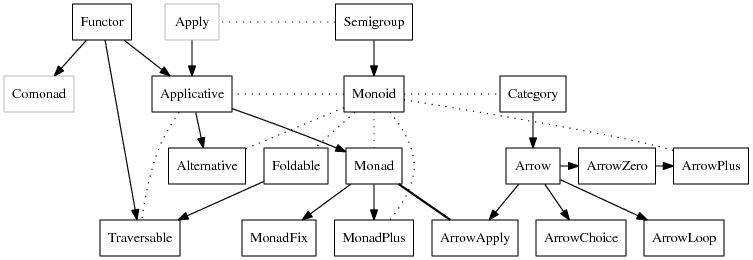
\includegraphics[width=1\textwidth]{figs/Typeclassopedia-diagram}
        \end{center}
    \end{frame}

    \sectionplan{Аппликативные функторы}
    
    \begin{frame}[fragile]{Больше, чем результат}
        \begin{block}{Moggi's principle}
            \begin{center}
                <<Computations of type $\alpha$ correspond to values of type $f\ap\alpha$>>
            \end{center}
        \end{block}
        %! suppress = EscapeUnderscore
        \begin{itemize}
            \item В чистом языке функция может только принять что-то и вернуть: $a\to b$
            \item А что если хочется сделать что-то ещё? --- породить \emph{эффект}
            \item Будем возвращать результат в коробочке с доп. информацией: $a\to f\ap b$
            \item[\eg] \mintinline{haskell}|Identity _| --- просто результат
            \item[\eg] \mintinline{haskell}|Maybe _| --- результата может не быть
            \item[\eg] \mintinline{haskell}|(w, _)| --- к результату есть доп. значение
            \item[\eg] \mintinline{haskell}|[_]| --- результатов может быть сколько угодно
            \item[\eg] \mintinline{haskell}|e -> _| --- для получения результата требуется доп. значение
        \end{itemize}
    \end{frame}

    \begin{frame}[fragile]{Аппликативные функторы для вычислений над содержимым коробочек}
        \begin{itemize}
            \item Применяя функции вида $a \to f \ap b$ получаем значения вида $f \ap b$
            \item Хотим продолжить делать вычисления над ними
            \item Нужен специальный код для каждого $f$, знающий как это делать
        \end{itemize}
        \pause
        \vspace{0.5em}
        \begin{minted}{haskell}
            class Applicative f where
              pure :: a -> f a
              liftA2 :: (a -> b -> c) -> f a -> f b -> f c
        \end{minted}
    \end{frame}
    
    \begin{frame}[fragile]{Аппликатив \mintinline{haskell}|Either|}
        \begin{minted}{haskell}
            class Applicative f where
              pure :: a -> f a
              liftA2 :: (a -> b -> c) -> f a -> f b -> f c
        \end{minted}
        \begin{itemize}
            \item[\todo] Реализуйте инстанс аппликатива для \mintinline{haskell}|Either|
            \item[\todo] По Id двух игроков, вычислите, у которого преимущество в игре
            \begin{minted}{haskell}
                data Player = Player { nick :: String, rank :: Int }
                dbLookup :: Db -> Id -> Either DbError Player
            \end{minted}
            \item[\todo] По двум командам игроков (пара списков Id) вычислите, у которой преимущество
            \item[\answer] \pause
            \begin{minted}{haskell}
                advantage :: Db -> [Id] -> [Id] -> Either DbError Bool
                advantage db ids1 ids2 = liftA2 (<) (teamRank ids1) (teamRank ids2) where
                  teamRank = fmap (sumBy rank) . liftAll (dbLookup db)
                  sumBy f = sum . map f

                liftAll :: Applicative f => (a -> f b) -> [a] -> f [b]
                liftAll f = foldr (liftA2 (:)) (pure []) . map f
            \end{minted}
        \end{itemize}
    \end{frame}

    \begin{frame}[fragile]{Аппликатив \mintinline{haskell}|(->)|}
        \begin{minted}{haskell}
            class Applicative f where
              pure :: a -> f a
              liftA2 :: (a -> b -> c) -> f a -> f b -> f c
        \end{minted}
        \begin{itemize}
            \item[\todo] Реализуйте инстанс аппликатива для функциональной стрелки
            \item[\todo] Найдите всех пользователей по Id в надёжной БД
            \begin{minted}{haskell}
                dbLookup :: Id -> Db -> Player
                liftAll :: Applicative f => (a -> f b) -> [a] -> f [b]
            \end{minted}
            \item[\answer] \pause
            \begin{minted}{haskell}
                lookupAll :: [Id] -> Db -> [Player]
                lookupAll = liftAll dbLookup
            \end{minted}
        \end{itemize}
    \end{frame}

    \begin{frame}[fragile]{Идиома вычислений в аппликативном контексте}
        \vspace{-0.5em}
        \begin{itemize}
            \item Хотим использовать функции произвольной арности
            \item Обобщим ``каррированной'' версией \mintinline{haskell}|liftA2| (на самом деле они эквивалентны)
            \begin{minted}{haskell}
                (<*>) :: Applicative f => f (a -> b) -> f a -> f b
            \end{minted}
            \item Теперь произвольный \mintinline{haskell}|liftAN| выражается однообразно
            \begin{minted}{haskell}
                liftA4 :: Applicative f => (a -> b -> c -> d -> r)
                                        -> (f a -> f b -> f c -> f d -> f r)
                liftA4 f a b c d = pure f <*> a <*> b <*> c <*> d
            \end{minted}
            \begin{itemize}
                \item \mintinline{haskell}|pure f      :: f (a -> b -> c -> d -> r)|
                \item \mintinline{haskell}|pure f <*> a     :: f (b -> c -> d -> r)|
                \item \mintinline{haskell}|pure f <*> a <*> b    :: f (c -> d -> r)|
                \item \mintinline{haskell}|pure f <*> a <*> b <*> c   :: f (d -> r)|
                \item \mintinline{haskell}|pure f <*> a <*> b <*> c <*> d  :: (f r)|
            \end{itemize}
            \item Боллее идеоматично пользоваться \texttt{pure f <*> x = f <\$> x}
        \end{itemize}
    \end{frame}

    \begin{frame}{\st{Death} Context parade \popslide}
        \begin{enumerate}
            \item Контекст типизации $\Gamma$ --- хранит типы переменных
            \item Контекст типа \mintinline{haskell}|(Ord a, Bounded a) =>| --- перечень ограничений (constraints) на типовые переменные в этом типе
            \item Вычислительный контекст \texttt{f} --- типовой конструктор, который объявлен представителем \mintinline{haskell}|Applicative|
            \item Контекст-окружение \mintinline{haskell}|e ->| --- константная конфигурация, распространяемая реализацией \mintinline{haskell}|Applicative| для функциональной стрелки
            \item Контекст зиппера --- части структуры данных, не находящиеся в фокусе зиппера
            \item и т.д.
        \end{enumerate}
        \vspace{0.5em}
        Так что слово ``контекст'' мы будем понимать по-разному в зависимости от контекста.
    \end{frame}
    
    \sectionplan{Композиция типов}

    \begin{frame}[fragile]{Функции на типах}
        \begin{itemize}
            \item[\todo] Как написать на типах \texttt{id}?
            \item[\answer] \pause
            \begin{itemize}
                \item Kind: \mintinline{haskell}|Id :: * -> *|
                \item Def: \mintinline{haskell}|type Id a = a|
            \end{itemize}
            \item[\todo] \pause Как написать на типах \texttt{flip}?
            \item[\answer] \pause
            \begin{itemize}
                \item Kind: \mintinline{haskell}|Flip :: (* -> * -> *) -> * -> * -> *|
                \item Def: \mintinline{haskell}|type Flip p a b = p b a|
            \end{itemize}
            \item[\todo] \pause Композиция типов?
            \item[\answer] \pause
            \begin{itemize}
                \item Kind: \mintinline{haskell}|Compose' :: (* -> *) -> (* -> *) -> * -> *|
                \item Def: \mintinline{haskell}|type Compose' f g a = f (g a)|
            \end{itemize}
            \item[\todo] \pause Композиция типов через \mintinline{haskell}|newtype|? В чем разница?
            \item[\answer] \pause
            %! suppress = EscapeHashOutsideCommand
            \begin{itemize}
                \item Def: \mintinline{haskell}|newtype Compose f g a = Compose (f (g a))|
                \item Пропала эквивалентность \mintinline{haskell}|Compose f g a #$\sim$# f (g a)|
                \item[\NB] Реализации классов типов ищутся для \mintinline{haskell}|Compose|, а не для \texttt{f}
            \end{itemize}
        \end{itemize}
    \end{frame}

    \begin{frame}[fragile]{Композиция типов}
        \vspace{-0.5em}
        \pause
        \begin{minted}{haskell}
            newtype Compose f g a = Compose { getCompose :: f (g a) }
        \end{minted}
        \begin{itemize}
            \item[\todo] \pause \mintinline{haskell}|GHCi> :t Compose [Just 42]|
            \item[\answer] \pause \mintinline{haskell}|Compose [] Maybe Int|
            \item[\todo] \pause \mintinline{haskell}|GHCi> :t Compose [Just [42]]|
            \item[\answer] \pause \mintinline{haskell}|Compose [] Maybe [Int]|
            \item[\todo] \pause \mintinline{haskell}|GHCi> :t Componse (Compose [Just [42]])|
            \item[\answer] \pause \mintinline{haskell}|Compose (Compose [] Maybe) [] Int|
        \end{itemize}
    \end{frame}

    \begin{frame}[fragile]{Композиция функторов --- функтор}
        \begin{itemize}
            \item[\todo] Докажите
            \item[\answer] \pause
            \begin{minted}{haskell}
                instance (Functor f, Functor g) => Functor (Compose f g) where
                  fmap :: (a -> b) -> Compose f g a  -> Compose f g b
                  --   :: (a -> b) -> f (g a)        -> f (g b)
                  fmap f = Compose . fmap (fmap f) . getCompose
            \end{minted}
            \item[\todo] \pause
            \begin{minted}{haskell}
                GHCi> length <\$> Compose [Just [42]]
            \end{minted}
            \item[\answer] \pause \mintinline{haskell}|Compose [Just 1] :: Compose [] Maybe Int|
        \end{itemize}
    \end{frame}

    \begin{frame}[fragile]{Композиция аппликативов --- аппликатив}
        \begin{itemize}
            \item[\todo] Докажите
            \item[\answer] \pause
            \begin{minted}{haskell}
                instance (Applicative f, Applicative g) => Applicative (Compose f g) where
                  pure = Compose . pure . pure
                  liftA2 op (Compose x) (Compose y) = liftA2 (liftA2 op) x y
            \end{minted}
            \item Теперь пример с игроками можно больше механизировать
            \begin{minted}{haskell}
                type Effs = Compose ((->) Db) (Either DbError)
                dbLookup :: Id -> Effs Player -- больше не передаём БД вручную
            \end{minted}
            \item[\NB] Аппликативные функторы позволяют замести под ковёр неинтересную рутину и церемонии, оставив нас наедине с бизнес-логикой
        \end{itemize}
    \end{frame}

    \sectionplan{Материалы}

    \begin{frame}[fragile]{Что посмотреть в транспорте}
        \begin{itemize}
            \item \href{https://youtu.be/n3H_YipBDrY?si=bsR5Fj56GEAIpAGE}{\color{blue} Vitaly Bragilevsky - The clear path to Haskell complexities}
            \item \href{https://youtu.be/MbFqJ2NHS8M?si=LamIrSnrjbwCYrt2}{\color{blue}  Tagless-Final Style}
        \end{itemize}
    \end{frame}

    \begin{frame}[fragile]{Серьёзные материалы}
        \begin{itemize}
            \item \href{https://www.staff.city.ac.uk/~ross/papers/Applicative.html}{\color{blue}Статья, вводящая аппликативы}
        \end{itemize}
    \end{frame}

\end{document}
